\section{Redes neuronales}

\begin{frame}\frametitle{Modelo de una neurona}
  \begin{figure}
    \centering
    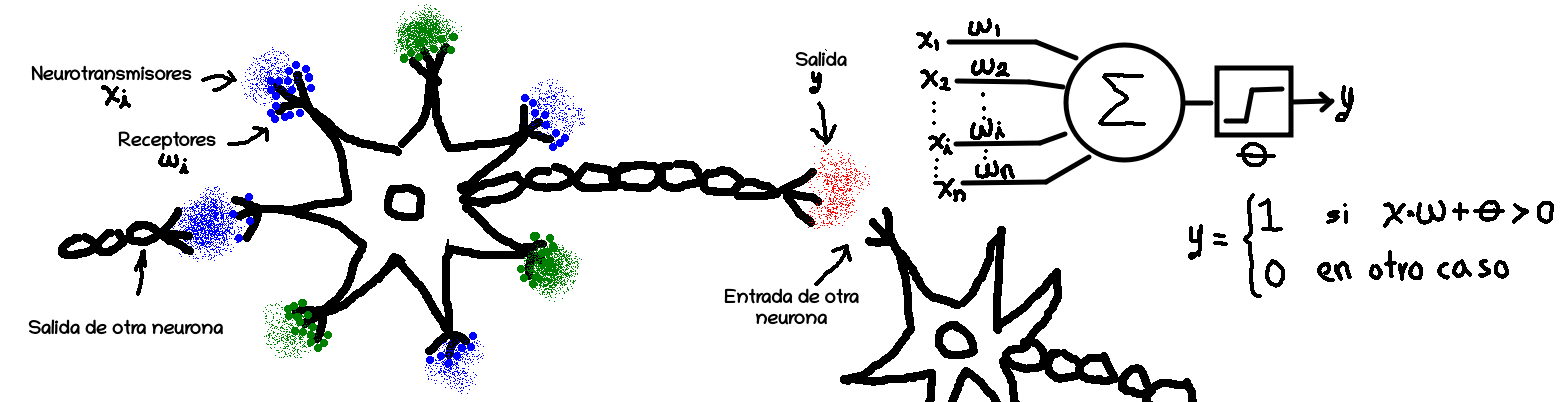
\includegraphics[height=0.4\textheight]{Figures/NN_Neurona.png}
  \end{figure}
  \begin{itemize}
  \item Una neurona tiene una diferencia de potencial entre el interior y exterior de la membrana de aprox -70 mV
  \item Los neurotransmisores abren canales para dejar pasar iones positivos o negativos por lo que hacen que el voltaje aumente o disminuya
  \item La efectividad del neurotransmisor depende de la cantidad de receptores en la membrana
  \item La cantidad de neurotransmisor se puede considerar como una señal de entrada $x_i$ que se pondera por la cantidad de receptores $w_i$
  \item Si el efecto de todos los neurotransmisores hace que el voltaje supere los -50 mV aprox, se produce un pulso eléctrico que hace que la neuorona libere neurotransmisor 
  \end{itemize}
  \begin{columns}
    \begin{column}{0.6\textwidth}
    \end{column}
    \begin{column}{0.4\textwidth}
      % \[y = \left\{\begin{array}{cl}
      %   1 & \textrm{si}\qquad w\cdot x + \theta > 0\\
      %   0 & \textrm{en otro caso}
      %   \end{array}\right.\]
    \end{column}
  \end{columns}
\end{frame}

\begin{frame}\frametitle{Ejemplos con compuertas}
  \begin{figure}
    \centering
    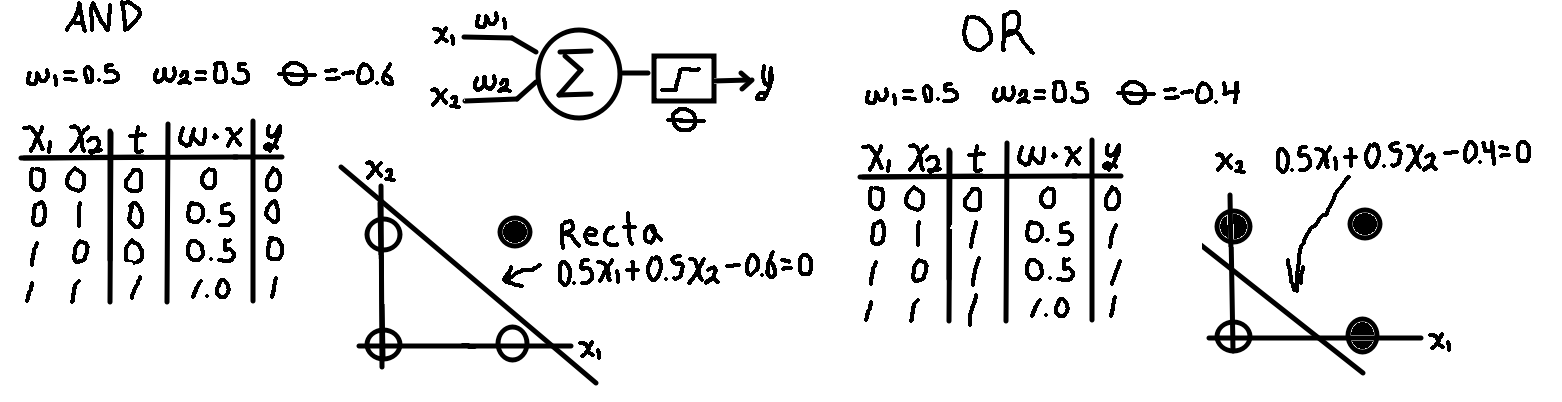
\includegraphics[width=\textwidth]{Figures/NN_AND_OR.png}
  \end{figure}
\end{frame}

\begin{frame}\frametitle{Separabilidad lineal}
\end{frame}

\begin{frame}\frametitle{Entrenamiento de una neurona}
\end{frame}

\begin{frame}\frametitle{Backpropagation}
  La red neuronal está definida por la cantidad de neuronas en cada capa $[l_0, l_1, \dots, l_{n-1}, l_n]$:
  
  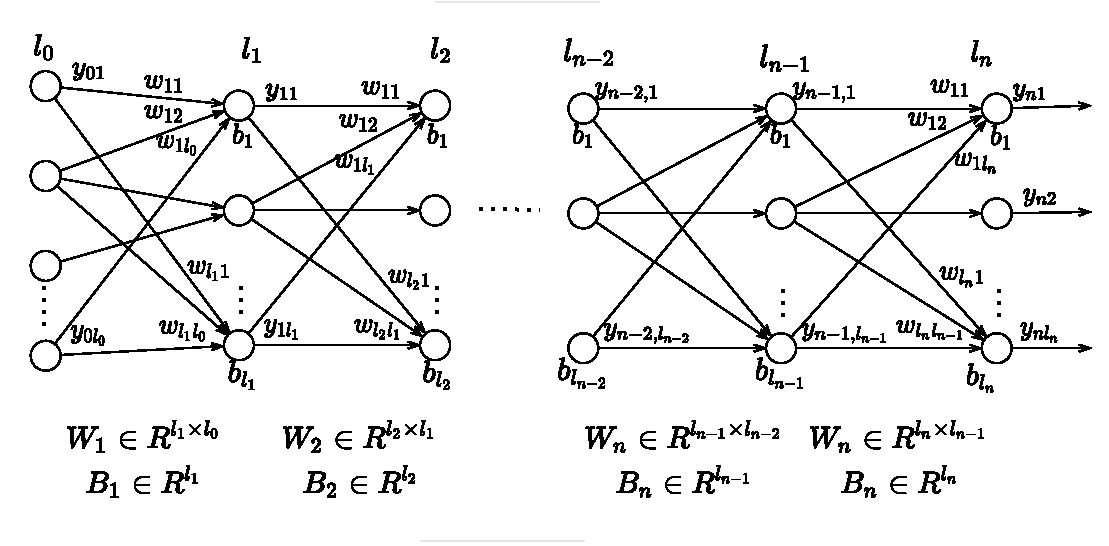
\includegraphics[width=0.9\textwidth]{Figures/NeuralNetworks1.pdf}
  
  El conjunto de pesos $w$ se puede agrupar en un conjunto de $n$ matrices $W=[W_1, W_2, \dots , W_n]$ con los órdenes indicados en la figura. El conjunto de biases se puede agrupar en $n$ vectores $B=[B_1, B_2, \dots, B_n]$. 
\end{frame}

\begin{frame}\frametitle{Backpropagation}
  Para la capa salida, el gradiente  con respecto a cada uno de los pesos $w\in W_n\in\mathbb{R}^{l_n\times l_{n-1}}$ es también una matriz $\nabla y_n \in \mathbb{R}^{l_n\times l_{n-1}}$:
  \[\left[\begin{tabular}{cccc}
      $(y_{n1} - t_1)(y_{n1}-y_{n1}^2)y_{n-1,1}$ & $(y_{n1} - t_1)(y_{n1}-y_{n1}^2)y_{n-1,2}$ & \dots & $(y_{n1} - t_1)(y_{n1}-y_{n1}^2)y_{n-1,l_{n-1}}$ \\
      $(y_{n2} - t_2)(y_{n2}-y_{n2}^2)y_{n-1,2}$ & $(y_{n2} - t_2)(y_{n2}-y_{n2}^2)y_{n-1,2}$ & \dots & $(y_{n1} - t_1)(y_{n1}-y_{n1}^2)y_{n-1,l_{n-1}}$ \\
  \end{tabular}\right]\]
\end{frame}

\begin{frame}\frametitle{Ejercicio 10 - Redes neuronales}
\end{frame}